\begin{appendices}
% \renewcommand{\theequation}{\thesection.\arabic{equation}}
% \clearpage
\section{Details of Experiments and Architectures}

\subsection{Internal Net $\mathcal{K}_\theta$}
Table.~\ref{tab:internal} below shows the architecture of the internal net $\mathcal{K}_\theta$ used for all experiments. The properties of each layer is denoted by  \textsc{Conv} $[Channels], [Kernel\_height] \times [Kernel\_width] + [Stride]$. Each Conv layer of  $\mathcal{K}_\theta$ except the last one, is followed by LeakyReLU activation. Each \CC layer contains its own \textsc{InternalNet}$: \mathbb{R}^2 \to \mathbb{R}$ (the learned continuous kernel). The input to \textsc{InternalNet} are distances from a specific pixel position in the output, given as a 4D tensor, and computed using $3$ consecutive 2D 1$\times$1 convolutions, as detailed in the table .

Block 2 in Sec.~\ref{sec:implement_construct} describes the input to $\mathcal{K}_\theta$ -- distances tensor of size $[K,2,H',W']$ where K is the number of neighbors within the support. When applying 2D conv layers to it, the first dimension of the tensor is regarded as the batch dimension. We do so intentionally, as we want to apply the same operation to all neighbor distances in parallel. The final calculated weight tensor is of size $[1,C_{out},C_{in},K,H',W']$, where $C_{in}, C_{out}$ are the numbers of input channels and output channels, respectively. 

By default, the number of channels of the final internal conv layer,  {$C_{final}$} needs to cover both in and out external channels of the CC layer. {$C_{final} = C_{in} \times C_{out}$}, then the calculated weights tensor  can be obtained by simple reshaping of the Internal Net's output: 
$[K, C_{out}\times C_{in}, H', W'] \rightarrow [1,C_{out},C_{in},K,H',W']$. 
In the equivariance experiment we used the efficient implementation mentioned in Sec.~\ref{sec:efficiency}: "No need to keep the Neighbors distances". In this case, the input is just the grid [1,2,H',W'] so the batch size is 1 and {$C_{final} = C_{in} \times C_{out} \times K$} to accommodate for the weights of all the neighbors.

\begin{table}[h!]
    \centering
    \begin{tabular}{lll}
    \toprule
       InternalNet  \\
    \midrule
      \textsc{Conv} 16 1x1+1  \\
      \textsc{Conv} 16 1x1+1  \\
      \textsc{Conv} $C_{final}$ 1x1+1  \\
    \bottomrule
    \end{tabular}
    \vspace{5pt}
    \caption{Architecture used for $\mathcal{K}_\theta$ in all experiments}
    \label{tab:internal}
\end{table}


% \subsection{Shift equivariance experiment -- Classification network architecture}
\subsection{Shift Equivariance Experiments}
All experiments were conducted on \textsc{CIFAR10} dataset \cite{CIFAR10} and implemented using \textsc{PyTorch}~\cite{paszke2017automatic} deep learning framework. 

The architectures we used for the Classification Networks in Sec.~\ref{sec:efficiency} are detailed in Table~\ref{tab:architectures}. \textsc{CC} corresponds to a continuous convolution layer with similar terminology (except that \textsc{CC} layers do not have a fixed stride). \textsc{FC} $n$ corresponds to a fully connected layer with $n$ outputs. Each \textsc{Conv}/\textsc{FC} layer is followed by a ReLU activation except for the last fully connected layer. As can be seen, \textsc{CCNet} and \textsc{ConvNet} share the same general architecture. The models are based on similar models from \cite{wong2018scaling,atzmon2019controlling}, where we added a few more convolution layers to exemplify the gradual change in scale.

\begin{table}[h!]
    \centering
    \begin{tabular}{lll}
    \toprule
         \textsc{ConvNet (Baseline)}  & \textsc{CCNet}\\
    \midrule
         \textsc{Conv} 32 3x3+1     & \CC 32 3x3      \\
         \textsc{Conv} 32 4x4+2     & \CC 32 4x4      \\
         \textsc{Conv} 64 3x3+1     & \CC 64 3x3      \\
         \textsc{Conv} 64 3x3+1     & \CC 64 3x3      \\
         \textsc{Conv} 64 3x3+1     & \CC 64 3x3      \\
         \textsc{Conv} 64 3x3+1     & \CC 64 3x3      \\
         \textsc{Conv} 64 3x3+1     & \CC 64 3x3      \\
         \textsc{Conv} 64 4x4+2     & \CC 64 4x4      \\
         \textsc{FC} 512            & \textsc{FC} 512 \\
         \textsc{FC} 512            & \textsc{FC} 512 \\
         \textsc{FC} 10             & \textsc{FC} 10  \\
    \bottomrule\\
    \end{tabular}
    \vspace{-5pt}
    \caption{Model architectures used for shift-equivariance experiment}
    \label{tab:architectures}
\end{table}


\paragraph{Initialization} The outputs of the \textsc{InternalNet} are equivalent to the weights of an ordinary \textsc{Conv} layer. At initialization, we require those outputs to have a variance similar to an ordinary \textsc{Conv} layer's weights at initialization (either \textit{Xavier} \cite{glorot2010understanding}, \textit{Kaiming} \cite{he2015delving} or the default \textsc{PyTorch}~\cite{paszke2017automatic} initializations). This is done by initializing the biases of the last layer of the \textsc{InternalNet} using a normal distribution with the required variance.

\paragraph{Training Hyperparameters} All models were trained using a batch size of $64$ of images obtained by padding the original CIFAR10 images by 8 rows/cols (4 from each side) and taking a random crop of $32 \times 32$. We also use
% images with random-crops of $32\times 32$ of images padded by 4 rows/cols (2 from each side), 
random horizontal-flip and normalize the inputs to have zero mean and unit variance (as done with common models for training on \textsc{CIFAR10}~\cite{pytorch-cifar}). 
We used \textsc{ADAM} optimizer \cite{kingma2014adam} with weight-decay of $0.0005$. For \textsc{CCNet} we use learning rate of $0.0005$ with a reduction by $10$ on epochs $[200,300]$. For the baseline \textsc{ConvNet} model we checked learning rates $0.0001, 0.0005, 0.001, 0.002$ with several learning rate scheduling (reducing by $10$) at: $[70,150], [150,250], [100,250], [200,300]$, with and without weight-decay, and chose the best performing model of learning rate $0.001$, weight-decay of $0.0005$ and learning rate reduction at epochs $[150,250]$. Results are reported after $400$ epochs, where all our runs seem to fully converge (e.g., further reduction in learning rates did not change the reported results).

\paragraph{Training and Inference with scale-augmentations} 
As mentioned, \CC layers can be given the scale and output shape dynamically during forward pass. In order to train a \textsc{CCNet} model with scale-augmentations we use the following design: the first \CC layer has a fixed scale of $1$ and output shape equal to input shape. We are left with $7$ \CC layers to reduce spatial dimension by $1/4$, that is, we want the product of all $7$ \CC layers' scales to equal to $1/4$. The \CC layers' scales are then sampled from a normal distribution of mean $(1/4)^{(1/7)}$ and standard deviation of $0.01$. All scales are then projected to the nearest rational fraction with a maximal denominator of $10$. At this point we have $7$ scales $\{s_i \}_{i=1}^7$, however $\Pi s_i$ does not necessarily equal to our target scale $1/4$. To this end we uniformly at random choose one layer $j$ and set $s_j = (1/4) / \Pi_{i \neq j} s_i$. At inference time we sample $k$ scales using the same methodology described here. The output shapes are determined by the following:
\begin{equation}
    \mathrm{output\_shape}\left(j\right) = \begin{cases} 
          \Bigl\lceil{\mathrm{input\_shape} \times \Pi_{i=1}^j s_i }\Bigr\rceil & j\mathrm{\ is\ not\ last} \\
          \mathrm{input\_shape} \times (1/4) & j \mathrm{\ is\ last\ layer} \\
   \end{cases}
   \label{eq:output_shape}
\end{equation}

A few examples for scale augmentations are shown in Table~\ref{tab:scale_augs_examples}.

\renewcommand{\arraystretch}{1.3}
\begin{table}[h!]
    \centering
    \begin{tabular}{l|cc|cc}
    \toprule
                & \multicolumn{2}{c}{Augmentation Example 1}                     & \multicolumn{2}{c}{Augmentation Example 2}                        \\
         Layer  &                {Scale [H,W]}                                & $\to$ Output Shape   & {Scale [H,W]} & $\to$ Output Shape         \\
    \midrule
        $1$     &                $[ \frac{1}{1}$    , $\frac{1}{1}]$          &   $[32,32]$          & $[\frac{1}{1}$  , $\frac{1}{1}]$     & $[32,32]$      \\        
        $2$     &                $[ \frac{5}{6}$    , $\frac{7}{9}]$          &   $[27,25]$          & $[\frac{75}{98}$, $\frac{7}{8}]$     & $[25,28]$      \\        
        $3$     &                $[ \frac{5}{6}$    , $\frac{4}{5}]$          &   $[23,20]$          & $[\frac{4}{5}$  , $\frac{2}{3}]$     & $[20,19]$      \\        
        $4$     &                $[ \frac{8}{9}$    , $\frac{5}{6}]$          &   $[20,17]$          & $[\frac{4}{5}$  , $\frac{3}{4}]$     & $[16,14]$      \\        
        $5$     &                $[ \frac{189}{250}$, $\frac{3}{4}]$          &   $[15,13]$          & $[\frac{7}{8}$  , $\frac{5}{6}]$     & $[14,12]$      \\        
        $6$     &                $[ \frac{6}{7}$    , $\frac{6}{7}]$          &   $[13,11]$          & $[\frac{5}{6}$  , $\frac{5}{6}]$     & $[12,10]$      \\        
        $7$     &                $[ \frac{5}{6}$    , $\frac{7}{8}]$          &   $[11,10]$          & $[\frac{7}{9}$  , $\frac{864}{875}]$ & $[9\ ,10]$      \\        
        $8$     &                $[ \frac{3}{4}$    , $\frac{6}{7}]$          &   $[8\ ,\ 8]$        & $[\frac{9}{10}$ , $\frac{5}{6}]$     & $[8\ ,\ 8]$    \\
    \bottomrule
    \end{tabular}
    \vspace{5pt}
    \caption{Examples of scale augmentations. $[H,W]$ corresponds to each spatial dimension. The model consists of $8$ continuous convolution layers (where the first is fixed to a scale $[1,1]$), input-shape is $[32,32]$ and target-scale is $[\nicefrac{1}{4},\nicefrac{1}{4}]$. The output shapes are computed from the scales and input shape using Equation~\ref{eq:output_shape}.}
    \label{tab:scale_augs_examples}
\end{table}

% \begin{figure}[h!]
%     \centering
%     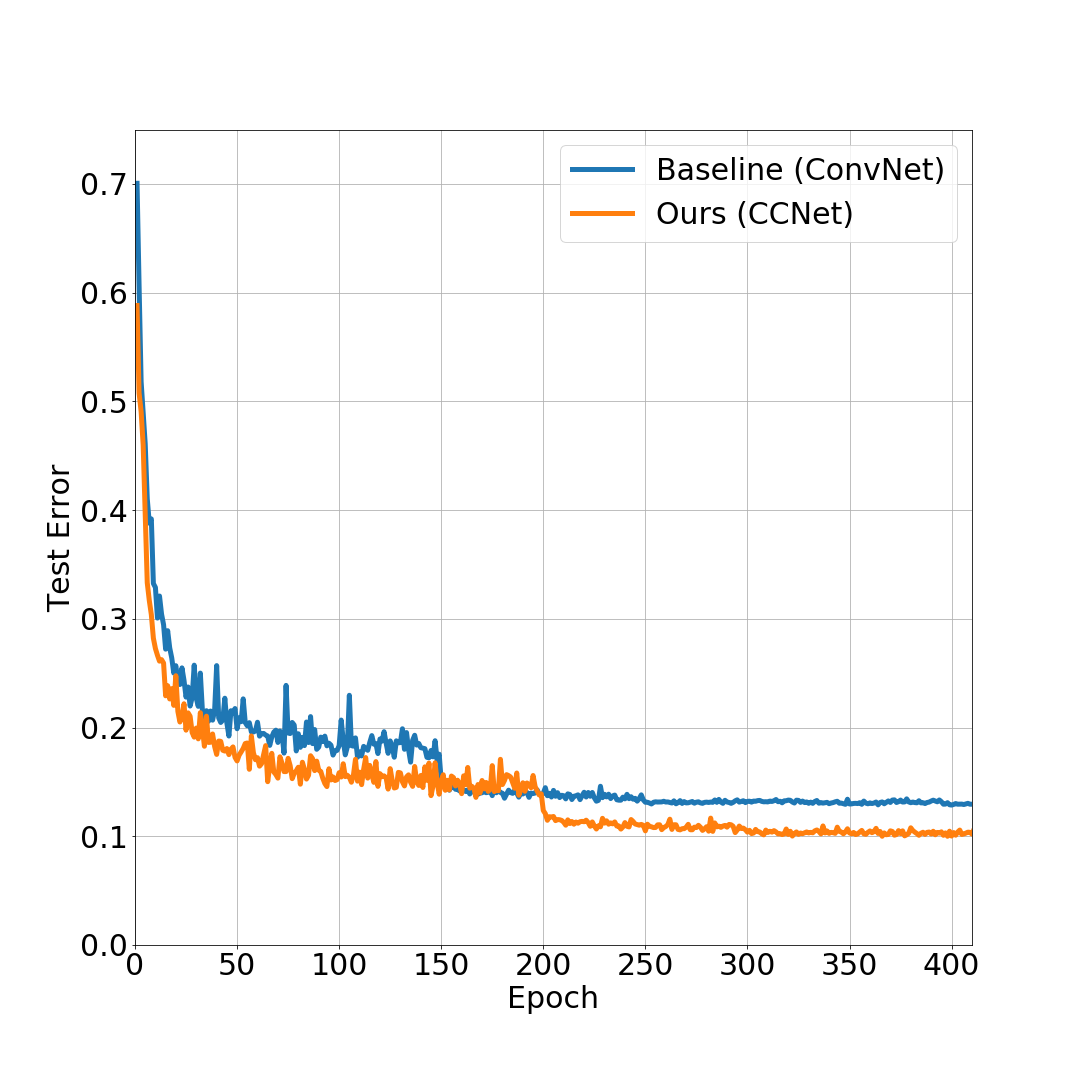
\includegraphics[width=0.65\columnwidth]{figs/classification_error.png}
%     \caption{Test error per epoch of our trained models}
%     \label{fig:training}
% \end{figure}

% \clearpage
\section{Runtime and Memory Analysis}
\subsection{CC Layers}
We measured the runtime and memory consumption of CC layers, with varying input size and number of consecutive layers. We show that our efficient implementation techniques (introduced in Sec.~\ref{sec:efficiency}) significantly reduce the memory footprint of a CC-layer, and some techniques (implementation using discrete convolutions) further speed up the layer. For reference, we also compare to a Conv-layer, although it lacks the expressiveness of the CC-layer. In the column ``CC (clear memory)'' (see Tables~\ref{tab:runtime_by_sz} and~\ref{tab:runtime_by_num_layers}), we divided the computation into chunks of size $32\times32$, computed the results sequentially and discarded all intermediate results (see "Saving memory by keeping only $\mathcal{K}_\theta$" in Sec.~\ref{sec:efficiency}). This implementation supports non-rational scales, and allows us to use deeper networks than the non-optimized implementation (``CC (standard)'' column). In the column ``CC (by discrete conv)'', the number of computed filters is reduced from the output size to the numerator of the scale factor -- in our case the scale factor is $\nicefrac{2}{3}$ so we have 2 filters. This mechanism is further optimized by using the convolution operation as backend (see "Efficient implementation using discrete convolutions" in Sec.~\ref{sec:efficiency}). This implementation significantly reduces memory consumption and runtime, at the cost of expressiveness -- as it only supports rational scale factors (and is beneficial as long as the numerator is small).

In terms of runtime, we measured the time of a single forward and backward pass through the layer (or layers). To accurately measure the time, we run 11 repeats and excluded the first (warm-up), and report the average of the last 10 (the deviation was negligible). In terms of memory consumption, we report the peak allocated memory in GiB ($2^{30}$ bytes). Sometimes there is a difference between the peak reserved memory and the peak allocated memory, but that's more related to the internals of \textsc{PyTorch}~\cite{paszke2017automatic}. All the tests were conducted on a single Tesla V100-PCIE-16GB GPU.

Table.~\ref{tab:runtime_by_sz} shows the runtime and memory consumption of a single layer with varying input size. In all the experiments we used a $3\times3$ kernel with 32 input channels and 32 output channels, and a batch size of 50. For the CC-layer, we used inner architecture as in Table.~\ref{tab:internal} with scale of $\nicefrac{2}{3}$. For the Conv-layer, we used stride of 1.

Table.~\ref{tab:runtime_by_num_layers} shows the runtime and memory consumption of multiple layers with a fixed input size of $64\times64$. In this experiment we used the same parameters, except for the scale -- here we used a scale of $1$ to have the same input size in all layers.

\begin{table}[h!]
    \centering
    \begin{tabular}{c|cccc}
    \toprule

Input Size     & CC (standard)     & CC (clear memory) & CC (by discrete convs) & Conv (reference) \\
\midrule
$32\times32$   & 8.7ms / 0.9GiB    & 19.7ms / 1.8GiB   & 3.5ms / 0.1GiB         & 0.8ms / 0.1GiB   \\
$64\times64$   & 30.0ms / 3.4GiB   & 76.1ms / 3.7GiB   & 3.6ms / 0.2GiB         & 1.3ms / 0.2GiB   \\
$96\times96$   & 72.3ms / 7.6GiB   & 155.4ms / 3.9GiB  & 5.1ms / 0.4GiB         & 2.7ms / 0.5GiB   \\
$128\times128$ & 131.5ms / 13.6GiB & 285.9ms / 4.1GiB  & 7.6ms / 0.7GiB         & 4.0ms / 0.4GiB   \\
    \bottomrule

    \end{tabular}
    \vspace{5pt}
    \caption{Runtime and memory consumption of CC-layer with varying input size.}
    \label{tab:runtime_by_sz}
\end{table}

\begin{table}[h!]
    \centering
    \begin{tabular}{c|cccc}
    \toprule
\# Layers & CC (standard)   & CC (clear memory) & CC (by discrete convs) & Conv (reference) \\
\midrule
1        & 71.7ms / 7.5GiB & 158.7ms / 3.8GiB  & 3.5ms / 0.3GiB         & 1.3ms / 0.2GiB   \\
2        & OUT OF MEMORY   & 317.9ms / 3.9GiB  & 7.0ms / 0.3GiB         & 2.8ms / 0.3GiB   \\
4        & OUT OF MEMORY   & 635.0ms / 4.0GiB  & 14.1ms / 0.4GiB        & 6.0ms / 0.4GiB   \\
8        & OUT OF MEMORY   & 1270.2ms / 4.2GiB & 27.1ms / 0.7GiB        & 12.5ms / 0.6GiB  \\
16       & OUT OF MEMORY   & 2538.7ms / 4.6GiB & 54.6ms / 1.1GiB        & 25.2ms / 1.0GiB  \\
32       & OUT OF MEMORY   & 5074.7ms / 5.5GiB & 111.3ms / 2.0GiB       & 51.6ms / 1.8GiB  \\
    \bottomrule
    \end{tabular}
    \vspace{5pt}
    \caption{Runtime and memory consumption of varying number of consecutive CC-layers.}
    \label{tab:runtime_by_num_layers}
\end{table}

\subsection{CC Classification Networks}
\textsc{Baseline ConvNet} takes 6 seconds per epoch, while \textsc{CCNet} takes 90 seconds per epoch. This difference is mainly attributed to the fact that CC-layer has a constant overhead of computing the weights, which is independent of the spatial size (when using conv implementation) and thus more significant when the input is small. Also, the feature maps in the \textsc{CCNet} are always (spatially) larger than in \textsc{Baseline ConvNet} due to the gradual downscaling. Finally, some scale factors (which were randomly chosen at each iteration) has large numerator which reduces the speed of the conv-based implementation.

\end{appendices}
